\chapter{Stop quark Production and Backgrounds}
\label{ch:Search}

In SUSY, spedifically the Minimally Supersymmetric Model (MSSM), the top squark $(\widetilde{t})$ is a bosonic superpartner to the top quark and should have a mass on the same scale as $t$. This is due to the strong mising between left and right superpartners to form eigenstates,

\begin{equation}
M_{\widetilde{q}}^2=
\begin{bmatrix}
\widetilde{M}_Q^2+M_Q^2+M_Z^2(\frac{1}{2}-\frac{2}{3}\sin^2\theta_W)\cos2\beta & M_Q(A_T+\frac{\mu}{\tan\beta}) \\
M_Q(A_T+\frac{\mu}{\tan\beta}) & \widetilde{M}_U^2+M_Q^2+\frac{2}{3}M_Z^2\sin^2\theta_W\cos2\beta
\end{bmatrix}
\end{equation}

This causes one of the \st to have one eigenstate that is the smallest for the quarks, see fig. 

\begin{figure}
\centering
	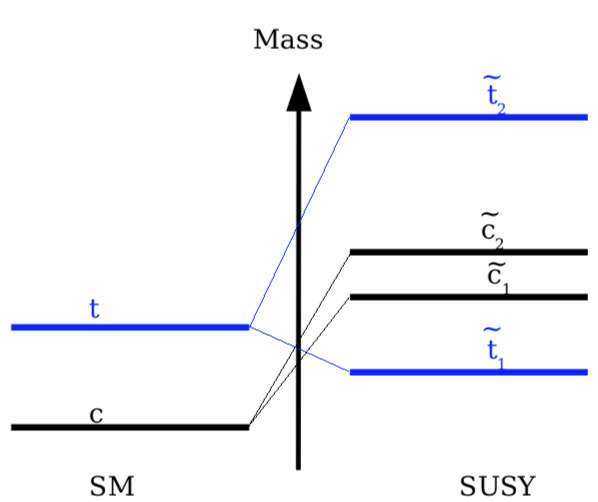
\includegraphics[width=0.5\textwidth]{TopSquarkMass.png}
 	\caption{On the right we have the arbitrary masses of the top and charm quarks.}
 	\label{StopMass} 
\end{figure}

\section{Production and Decay Modes}
\label{sec:Production}

Gluon fusion.

Main decay mode mode $\tilde{t}\rightarrow t+\tilde{\chi}^{0}_{1}$, $\tilde{t}\rightarrow b+\tilde{\chi}^{+}$. The top quark most likely decays into a b quark and W boson. 

\section{Standard Model Background}
\label{sec:SMBackground}

Signal events can be mimicked by SM events that have a large number of jets and missing energy. 

Broken up into four major backgrounds, Lost Lepton (LL), Znunu, QCD, Rare decays

\subsection{Lost Lepton}
\label{subsec:LL}

\ttbar{} production of ttbar via the same mechanism as stop-antistop which can be gluon fusion. They then decay the same why as explained above.

$W+$jets: Production of W bosons plus jets. Jets can be tagged as b jets. W boson decay hadronically or leptonically (where the lepton is missed)

tW and ttW: Missed lepton

\subsubsection{Transfer Factors}
\label{subsec:TF}

We want to suppress signal contamination by requiring $M_{T}(l, \met) < 100$ GeV. This requirement confirms that it is orthogonal to the search reagions that are used in the search for direct top squark production in the single-lepton final state. Letting the two anaysis statistically combine the results in the future. 

We are looking at the event count of data in each corresponding CR for the single-lepton sample. The prediction is allowed by means of a transfer factor (TF) which is obtained from simulation,

\begin{equation}
\label{eqn:LLTF}
N_{pred}^{LL}=TF_{LL} \cdot N_{data}(1l).
\end{equation}

This allows us to have the same selection for the single-lepton control sample and the zero-lepton sample. The only exception is the number of top and W-tagged candidates? what is the difference betweeen a candidate and a particle?

The LL estimation is dependent on the yield of data in the corresponding CR and the TF calculated by the single-lepton sample. The transfer factor is defined as, 

\begin{equation}
\label{eqn:TF}
TF_{LL}=\frac{N_{MC}(0l)}{N_{MC}(1l)},
\end{equation}

where $N_{MC}(1l)$ is the event count observed in the corresponding CR and $N_{MC}(0l)$ use the event count in the corresponding SR. 

\subsection{Z Boson Decay to Neutrinos}
\label{subsec:Znunu}

Znunu: production of a Z boson that decays into two nuetrinos which are then missed by the detector. Can have jets from other quarks/gluons in the interaction

\subsection{Quantum Chromodynamic Events}
\label{subsec:QCD}

QCD: Events that of jets produced by QCD processes. The missing energy from from a mismeasurement of the jets in the event causing missing energy

\subsection{Rare Interactions}
\label{subsec:rare}

ttZ, ttH, WW, WZ, ZZ, tZq, tWZ: rare processed that can have jets plus MET. Expand upon these later
